\documentclass[twocolumn]{article}

\usepackage[utf8]{inputenc}
\usepackage[T2A]{fontenc}
\usepackage[russian]{babel}
\usepackage{ragged2e}

\usepackage{amssymb}
\usepackage{graphicx}
\usepackage{fancyhdr}  


\pagestyle{fancy}  
\renewcommand{\headrulewidth}{0pt}    
\rhead{\bfseries http://kvant.mccme.ru}  

\fancyfoot[C]{}
\fancyfoot[L]{2*} % добавить 2* слева
\fancyfoot[R]{\textbf{19}} % добавить жирную 19 справа



\begin{document}


2. Пусть $A$, $B$, $C$ и $D$ - четыре произвольные точки плоскости. Тогда


$$(\sin^{2}\frac{\measuredangle ADB}{2}+\sin^{2}\frac{\measuredangle ADС}{2}-$$
$$-sin^{2}\frac{\measuredangle BDC}{2})^{2}=4\sin^{2}\frac{\measuredangle ADB}{2}\times$$
$$\times\sin^{2}\frac{\measuredangle ADС}{2}\times\cos{2}\frac{\measuredangle BDС}{2}$$



Доказательство. Возможны четыре случая взаимного расположения точек $A$, $B$, $C$ и $D$. В каждом из них выберем $U$, $V$ и $W$ в соответствии с таблицей, помещенной ниже. В любом случае $U \ge  0$, $V \ge  0$, $W \ge 0$ и $U + V + W = \pi$, так что, согласно пункту 1, 

$$(sin^{2}V + sin^{2}W - sin^{2}U)^2$$
$$= -4 sin^2 V \cdot  sin^2 W \cdot  cos^2 U$$

Остается воспользоваться тем, что в любом случае

$$sin U = sin^2 \frac{\measuredangle BDC}{2},$$
$$sin V = sin^2 \frac{\measuredangle ADC}{2},$$
$$sin W = sin^2 \frac{\measuredangle ADV}{2},$$
$$cos U = cos^2 \frac{\measuredangle BDC}{2}.$$

\begin{figure}
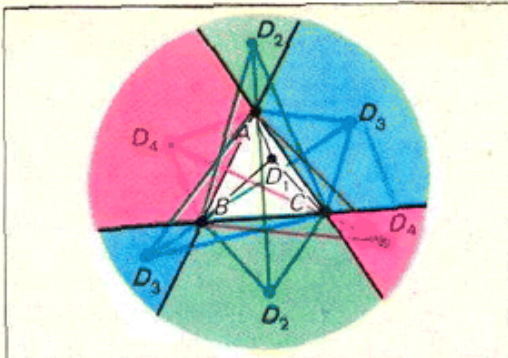
\includegraphics[width=0.45\textwidth]{рис8.png}
Рис. 8
\end{figure}

3. Пусть один из углов равен $\theta$, противоположная сто-

\begin{table}[b]
\centering
\renewcommand{\arraystretch}{1.7}
\begin{tabular}
{|c|p{7.5cm}|p{7.5cm}|}
\hline
\centering№ & Если & То \\
\hline
1 & $\measuredangle BDC +\measuredangle ADC + \measuredangle ADB =2\Pi$ & $U = \frac{\measuredangle BDC}{2},  V =\frac{\measuredangle ADC}{2}, W =\frac{\measuredangle ADB}{2}$ \\
\hline
2 & $\measuredangle BDC = \measuredangle ADC + \measuredangle ADB $ & $U = \Pi - \frac{\measuredangle BDC}{2},  V =\frac{\measuredangle ADC}{2}, W =\frac{\measuredangle ADB}{2}$ \\
\hline
3 & $\measuredangle ADC = \measuredangle ADB + \measuredangle BDC$ & $U =\frac{\measuredangle BDC}{2},  V = \Pi - \frac{\measuredangle ADC}{2}, W =\frac{\measuredangle ADB}{2}$ \\
\hline
4 & $\measuredangle ADB = \measuredangle BDC + \measuredangle ADC$ & $U =\frac{\measuredangle BDC}{2},  V =\frac{\measuredangle ADC}{2}, W =\Pi - \frac{\measuredangle ADB}{2}$ \\
\hline

\end{tabular}
\end{table}


\begin{minipage}[t]{\columnwidth}
рона - $u$, прилежащие - $v$ и $w$, полупериметр треугольника - $q$. Тогда

$$\cos^{2}\frac{\theta}{2}=\frac{q(q-u)}{v \cdot w}, \sin^{2}\frac{\theta}{2}=$$

$$=\frac{(q-v)(q-w)}{v \cdot w}$$

Доказательство. По теореме косинусов

$$u^2 = v^2 + w^2 - 2vw \cos \theta,\cos \theta =$$
$$=(v^2+w^2-u^2)/2vw.$$.

Значит,
$$\cos^{2}\frac{\theta}{2} =\frac{1+\cos\theta}{2}=\frac{(v^2+w^2)-u^2}{4v \cdot w} =$$

$$=\frac{(v+w+u)(v+w-u)}{4v \cdot w} = \frac{q(q-u)}{v \cdot w},$$
\end{minipage}
\end{document}
